\documentclass[border=10pt]{standalone}
\usepackage{tikz}
\usepackage[utf8]{inputenc}
\usepackage[T1]{fontenc}
\usetikzlibrary{patterns, decorations.pathreplacing, calc, arrows.meta}

\begin{document}
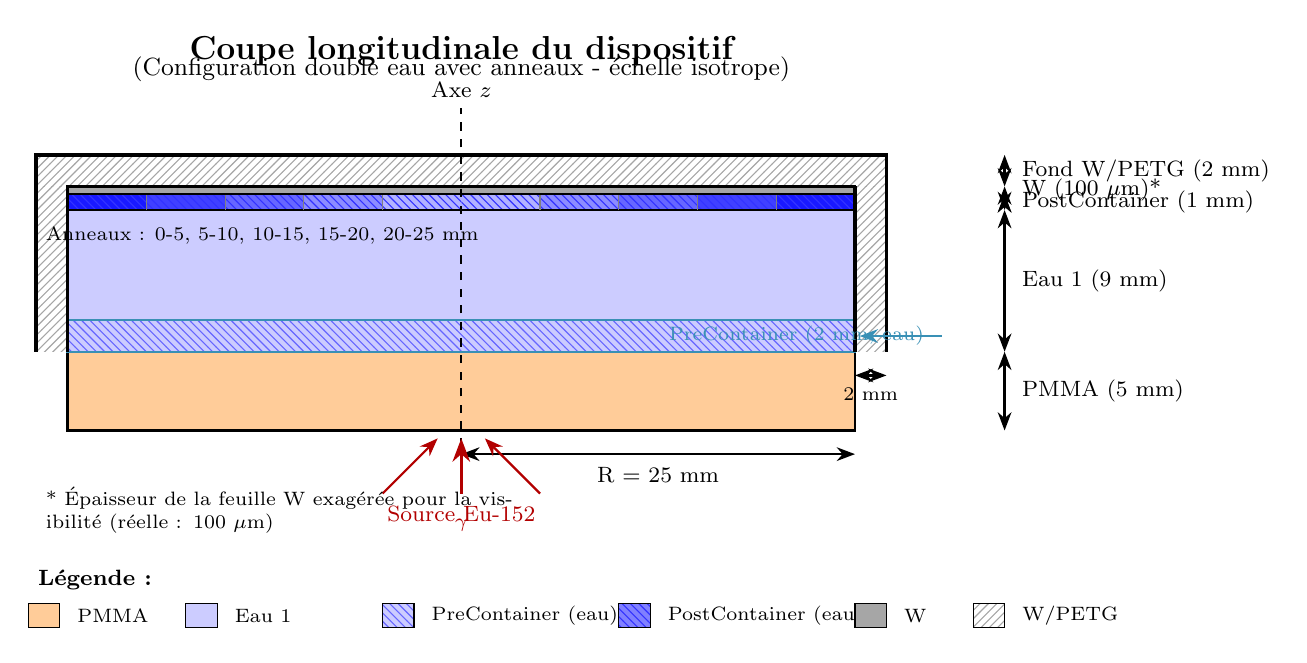
\begin{tikzpicture}[
    scale=1,
    >=Stealth,
    % Styles pour les matériaux
    pmma/.style={fill=orange!40},
    water1/.style={fill=blue!20},
    water2/.style={fill=blue!50},
    precontainer/.style={fill=blue!20, pattern=north west lines, pattern color=blue!60},
    tungsten/.style={fill=gray!70},
    wpetg/.style={fill=gray!50, pattern=north east lines, pattern color=gray!70},
    air/.style={fill=white},
]

% ============================================================
% ÉCHELLE ISOTROPE : 1 unité graphique = 5 mm
% ============================================================
\def\scale{0.2}  % 1 mm = 0.2 unités graphiques

% ============================================================
% PARAMÈTRES GÉOMÉTRIQUES (en mm)
% ============================================================
\def\containerInnerRadius{25}      % Rayon intérieur container
\def\containerWallThickness{2}     % Épaisseur parois (identique en r et z)
\def\containerInnerHeight{12}      % Hauteur intérieure container

\def\pmmaThickness{5}              % Épaisseur PMMA
\def\pmmaRadius{25}                % Rayon PMMA

\def\waterThicknessOne{9}          % Première tranche d'eau
\def\waterThicknessTwo{1}          % Deuxième tranche d'eau (anneaux)

\def\preContainerThickness{2}      % Épaisseur PreContainerPlane

\def\tungstenFoilThickness{0.1}    % Feuille W (100 µm)
\def\tungstenFoilThicknessVis{0.5} % Épaisseur visuelle (agrandie pour visibilité)

\def\ringWidth{5}                  % Largeur des anneaux

% Position Z de référence (bas du PMMA)
\def\zBasePMMA{0}

% Calcul des positions Z
\pgfmathsetmacro{\zTopPMMA}{\zBasePMMA + \pmmaThickness}
\pgfmathsetmacro{\zTopWaterOne}{\zTopPMMA + \waterThicknessOne}
\pgfmathsetmacro{\zTopWaterTwo}{\zTopWaterOne + \waterThicknessTwo}
\pgfmathsetmacro{\zTopTungsten}{\zTopWaterTwo + \tungstenFoilThicknessVis}
\pgfmathsetmacro{\zTopContainer}{\zTopTungsten + \containerWallThickness}

\pgfmathsetmacro{\containerOuterRadius}{\containerInnerRadius + \containerWallThickness}

% ============================================================
% DESSIN DE LA COUPE AVEC ÉCHELLE ISOTROPE
% ============================================================

% ============================================================
% FOND ET PAROIS DU CONTAINER W/PETG
% ============================================================

% Paroi latérale gauche
\fill[wpetg] 
    ({-\containerOuterRadius*\scale}, {\zTopPMMA*\scale}) rectangle 
    ({-\containerInnerRadius*\scale}, {\zTopTungsten*\scale});

% Paroi latérale droite
\fill[wpetg] 
    ({\containerInnerRadius*\scale}, {\zTopPMMA*\scale}) rectangle 
    ({\containerOuterRadius*\scale}, {\zTopTungsten*\scale});

% Fond du container (en haut)
\fill[wpetg] 
    ({-\containerOuterRadius*\scale}, {\zTopTungsten*\scale}) rectangle 
    ({\containerOuterRadius*\scale}, {\zTopContainer*\scale});

% ============================================================
% PMMA
% ============================================================
\fill[pmma] 
    ({-\pmmaRadius*\scale}, {\zBasePMMA*\scale}) rectangle 
    ({\pmmaRadius*\scale}, {\zTopPMMA*\scale});

% ============================================================
% PREMIÈRE TRANCHE D'EAU (9 mm) - uniforme
% ============================================================
\fill[water1] 
    ({-\containerInnerRadius*\scale}, {\zTopPMMA*\scale}) rectangle 
    ({\containerInnerRadius*\scale}, {\zTopWaterOne*\scale});

% ============================================================
% PRECONTAINER PLANE (2 mm) - à l'entrée de Water1
% ============================================================
\fill[precontainer] 
    ({-\containerInnerRadius*\scale}, {\zTopPMMA*\scale}) rectangle 
    ({\containerInnerRadius*\scale}, {(\zTopPMMA + \preContainerThickness)*\scale});

% ============================================================
% DEUXIÈME TRANCHE D'EAU (1 mm) - avec anneaux concentriques
% ============================================================

% Dessiner les 5 anneaux avec des couleurs différentes et des hachures (PostContainer)
\foreach \i in {0,1,2,3,4} {
    \pgfmathsetmacro{\rIn}{\i * \ringWidth}
    \pgfmathsetmacro{\rOut}{(\i + 1) * \ringWidth}
    \pgfmathsetmacro{\blueIntensity}{30 + \i * 15}
    
    % Anneau côté gauche (r négatif) - fond bleu + hachures
    \fill[fill=blue!\blueIntensity] 
        ({-\rOut*\scale}, {\zTopWaterOne*\scale}) rectangle 
        ({-\rIn*\scale}, {\zTopWaterTwo*\scale});
    \fill[pattern=north west lines, pattern color=blue!80] 
        ({-\rOut*\scale}, {\zTopWaterOne*\scale}) rectangle 
        ({-\rIn*\scale}, {\zTopWaterTwo*\scale});
    
    % Anneau côté droit (r positif) - fond bleu + hachures
    \fill[fill=blue!\blueIntensity] 
        ({\rIn*\scale}, {\zTopWaterOne*\scale}) rectangle 
        ({\rOut*\scale}, {\zTopWaterTwo*\scale});
    \fill[pattern=north west lines, pattern color=blue!80] 
        ({\rIn*\scale}, {\zTopWaterOne*\scale}) rectangle 
        ({\rOut*\scale}, {\zTopWaterTwo*\scale});
}

% ============================================================
% FEUILLE DE TUNGSTÈNE (100 µm) - épaisseur exagérée pour visibilité
% ============================================================
\fill[tungsten] 
    ({-\pmmaRadius*\scale}, {\zTopWaterTwo*\scale}) rectangle 
    ({\pmmaRadius*\scale}, {\zTopTungsten*\scale});

% ============================================================
% CONTOURS
% ============================================================

% Contour PMMA
\draw[thick] 
    ({-\pmmaRadius*\scale}, {\zBasePMMA*\scale}) rectangle 
    ({\pmmaRadius*\scale}, {\zTopPMMA*\scale});

% Contour Water1
\draw[thick] 
    ({-\containerInnerRadius*\scale}, {\zTopPMMA*\scale}) rectangle 
    ({\containerInnerRadius*\scale}, {\zTopWaterOne*\scale});

% Contour PreContainerPlane
\draw[thick, cyan!70!black] 
    ({-\containerInnerRadius*\scale}, {\zTopPMMA*\scale}) rectangle 
    ({\containerInnerRadius*\scale}, {(\zTopPMMA + \preContainerThickness)*\scale});

% Contour Water2 (anneaux)
\draw[thick] 
    ({-\containerInnerRadius*\scale}, {\zTopWaterOne*\scale}) rectangle 
    ({\containerInnerRadius*\scale}, {\zTopWaterTwo*\scale});

% Séparations des anneaux
\foreach \i in {1,2,3,4} {
    \pgfmathsetmacro{\rSep}{\i * \ringWidth}
    \draw[thin, gray] 
        ({-\rSep*\scale}, {\zTopWaterOne*\scale}) -- 
        ({-\rSep*\scale}, {\zTopWaterTwo*\scale});
    \draw[thin, gray] 
        ({\rSep*\scale}, {\zTopWaterOne*\scale}) -- 
        ({\rSep*\scale}, {\zTopWaterTwo*\scale});
}

% Contour feuille W
\draw[thick] 
    ({-\pmmaRadius*\scale}, {\zTopWaterTwo*\scale}) rectangle 
    ({\pmmaRadius*\scale}, {\zTopTungsten*\scale});

% Contour container
\draw[very thick] 
    ({-\containerOuterRadius*\scale}, {\zTopPMMA*\scale}) -- 
    ({-\containerOuterRadius*\scale}, {\zTopContainer*\scale}) -- 
    ({\containerOuterRadius*\scale}, {\zTopContainer*\scale}) -- 
    ({\containerOuterRadius*\scale}, {\zTopPMMA*\scale});

\draw[very thick] 
    ({-\containerInnerRadius*\scale}, {\zTopPMMA*\scale}) -- 
    ({-\containerInnerRadius*\scale}, {\zTopTungsten*\scale});
\draw[very thick] 
    ({\containerInnerRadius*\scale}, {\zTopPMMA*\scale}) -- 
    ({\containerInnerRadius*\scale}, {\zTopTungsten*\scale});

% ============================================================
% AXE DE SYMÉTRIE
% ============================================================
\draw[dashed, thick] (0, {-1*\scale}) -- (0, {(\zTopContainer + 3)*\scale});
\node[anchor=south] at (0, {(\zTopContainer + 3)*\scale}) {\footnotesize Axe $z$};

% ============================================================
% COTATIONS ET ANNOTATIONS
% ============================================================

% Position des annotations à droite
\pgfmathsetmacro{\annotX}{\containerOuterRadius*\scale + 1.5}

% PMMA
\draw[<->, thick] ({\annotX}, {\zBasePMMA*\scale}) -- ({\annotX}, {\zTopPMMA*\scale});
\node[anchor=west, font=\footnotesize] at ({\annotX + 0.1}, {(\zBasePMMA + \pmmaThickness/2)*\scale}) {PMMA (5 mm)};

% Water1
\draw[<->, thick] ({\annotX}, {\zTopPMMA*\scale}) -- ({\annotX}, {\zTopWaterOne*\scale});
\node[anchor=west, font=\footnotesize] at ({\annotX + 0.1}, {(\zTopPMMA + \waterThicknessOne/2)*\scale}) {Eau 1 (9 mm)};

% PreContainerPlane annotation
\draw[->, thick, cyan!70!black] ({\annotX - 0.8}, {(\zTopPMMA + \preContainerThickness/2)*\scale}) -- 
    ({(\containerInnerRadius + 0.3)*\scale}, {(\zTopPMMA + \preContainerThickness/2)*\scale});
\node[anchor=east, font=\scriptsize, cyan!70!black] at ({\annotX - 0.9}, {(\zTopPMMA + \preContainerThickness/2)*\scale}) {PreContainer (2 mm, eau)};

% Water2 = PostContainer
\draw[<->, thick] ({\annotX}, {\zTopWaterOne*\scale}) -- ({\annotX}, {\zTopWaterTwo*\scale});
\node[anchor=west, font=\footnotesize] at ({\annotX + 0.1}, {(\zTopWaterOne + \waterThicknessTwo/2)*\scale}) {PostContainer (1 mm)};

% Feuille W
\draw[<->, thick] ({\annotX}, {\zTopWaterTwo*\scale}) -- ({\annotX}, {\zTopTungsten*\scale});
\node[anchor=west, font=\footnotesize] at ({\annotX + 0.1}, {(\zTopWaterTwo + \tungstenFoilThicknessVis/2)*\scale}) {W (100 $\mu$m)*};

% Fond container
\draw[<->, thick] ({\annotX}, {\zTopTungsten*\scale}) -- ({\annotX}, {\zTopContainer*\scale});
\node[anchor=west, font=\footnotesize] at ({\annotX + 0.1}, {(\zTopTungsten + \containerWallThickness/2)*\scale}) {Fond W/PETG (2 mm)};

% Cotation paroi latérale
\draw[<->, thick] ({\containerInnerRadius*\scale}, {(\zTopPMMA - 1.5)*\scale}) -- 
    ({\containerOuterRadius*\scale}, {(\zTopPMMA - 1.5)*\scale});
\node[anchor=north, font=\scriptsize] at ({(\containerInnerRadius + \containerWallThickness/2)*\scale}, {(\zTopPMMA - 1.7)*\scale}) {2 mm};

% Rayon intérieur
\draw[<->, thick] (0, {(\zBasePMMA - 1.5)*\scale}) -- ({\containerInnerRadius*\scale}, {(\zBasePMMA - 1.5)*\scale});
\node[anchor=north, font=\footnotesize] at ({\containerInnerRadius*\scale/2}, {(\zBasePMMA - 1.7)*\scale}) {R = 25 mm};

% ============================================================
% LÉGENDE DES ANNEAUX
% ============================================================
\node[anchor=north west, font=\scriptsize] at ({-\containerOuterRadius*\scale}, {\zTopWaterOne*\scale - 0.1}) {Anneaux : 0-5, 5-10, 10-15, 15-20, 20-25 mm};

% ============================================================
% DIRECTION DES GAMMAS (SOURCE)
% ============================================================
\draw[->, very thick, red!70!black] (0, {(\zBasePMMA - 4)*\scale}) -- (0, {(\zBasePMMA - 0.5)*\scale});
\draw[->, thick, red!70!black] (-1, {(\zBasePMMA - 4)*\scale}) -- (-0.3, {(\zBasePMMA - 0.5)*\scale});
\draw[->, thick, red!70!black] (1, {(\zBasePMMA - 4)*\scale}) -- (0.3, {(\zBasePMMA - 0.5)*\scale});
\node[anchor=north, font=\footnotesize, red!70!black] at (0, {(\zBasePMMA - 4.2)*\scale}) {Source Eu-152};
\node[anchor=north, font=\scriptsize, red!70!black] at (0, {(\zBasePMMA - 5)*\scale}) {$\gamma$};

% ============================================================
% TITRE
% ============================================================
\node[anchor=south, font=\large\bfseries] at (0, {(\zTopContainer + 5)*\scale}) {Coupe longitudinale du dispositif};
\node[anchor=south, font=\small] at (0, {(\zTopContainer + 4)*\scale}) {(Configuration double eau avec anneaux - échelle isotrope)};

% ============================================================
% NOTE SUR L'ÉCHELLE
% ============================================================
\node[anchor=north west, font=\scriptsize, text width=6cm] at ({-\containerOuterRadius*\scale}, {(\zBasePMMA - 3)*\scale}) 
    {* Épaisseur de la feuille W exagérée pour la visibilité (réelle : 100 $\mu$m)};

% ============================================================
% LÉGENDE DES MATÉRIAUX
% ============================================================
\begin{scope}[shift={(-5.5, -2.5)}]
    \node[anchor=west, font=\footnotesize\bfseries] at (0, 0.6) {Légende :};
    
    \fill[pmma] (0, 0) rectangle (0.4, 0.3);
    \draw (0, 0) rectangle (0.4, 0.3);
    \node[anchor=west, font=\scriptsize] at (0.5, 0.15) {PMMA};
    
    \fill[water1] (2, 0) rectangle (2.4, 0.3);
    \draw (2, 0) rectangle (2.4, 0.3);
    \node[anchor=west, font=\scriptsize] at (2.5, 0.15) {Eau 1};
    
    \fill[blue!20] (4.5, 0) rectangle (4.9, 0.3);
    \fill[pattern=north west lines, pattern color=blue!60] (4.5, 0) rectangle (4.9, 0.3);
    \draw (4.5, 0) rectangle (4.9, 0.3);
    \node[anchor=west, font=\scriptsize] at (5, 0.15) {PreContainer (eau)};
    
    \fill[blue!50] (7.5, 0) rectangle (7.9, 0.3);
    \fill[pattern=north west lines, pattern color=blue!80] (7.5, 0) rectangle (7.9, 0.3);
    \draw (7.5, 0) rectangle (7.9, 0.3);
    \node[anchor=west, font=\scriptsize] at (8, 0.15) {PostContainer (eau)};
    
    \fill[tungsten] (10.5, 0) rectangle (10.9, 0.3);
    \draw (10.5, 0) rectangle (10.9, 0.3);
    \node[anchor=west, font=\scriptsize] at (11, 0.15) {W};
    
    \fill[wpetg] (12, 0) rectangle (12.4, 0.3);
    \draw (12, 0) rectangle (12.4, 0.3);
    \node[anchor=west, font=\scriptsize] at (12.5, 0.15) {W/PETG};
\end{scope}

\end{tikzpicture}
\end{document}
